\documentclass[11pt]{article}

% Change "review" to "final" to generate the final (sometimes called camera-ready) version.
% Change to "preprint" to generate a non-anonymous version with page numbers.
\usepackage[review]{acl}

\usepackage{times}
\usepackage{latexsym}
\usepackage[T1]{fontenc}
\usepackage[utf8]{inputenc}
\usepackage{microtype}
\usepackage{inconsolata}
\usepackage{graphicx}
\usepackage{booktabs}
\usepackage{algorithm}
\usepackage{algpseudocode}
\usepackage{amsmath}
\usepackage{amssymb}
\usepackage{tikz}
\usetikzlibrary{positioning,arrows.meta,shapes.geometric,calc}
\usepackage{amsthm}
\newtheorem{proposition}{Proposition}
\newtheorem{theorem}{Theorem}
\newtheorem{corollary}{Corollary}

\title{Dgrammar: Efficient Constrained Decoding for DLMs}

\author{Anonymous \\
  Anonymous Affiliation \\
  \texttt{anonymous@anonymous} \\}

\begin{document}
\maketitle

\begin{abstract}
Grammar-constrained decoding for DLMs remains slow because existing decoders enforce constraints one token at a time, turning violations into rejection, lookahead verification, or autoregressive fallback. This discards the block-parallel decoding advantage of DLMs. We introduce Dgrammar, which preserves multi-token unmasking and repairs violations in place under the same forward-pass logits. Dgrammar combines incremental prefix checking, selective remasking via logit truncation, asynchronous mask construction, and grammar-guided tail completion. We also characterize how rejection filtering, lookahead verification, and AR fallback change the model's scoring distribution. On JSONSchemaBench medium\_test with LLaDA-8B-Instruct, Dgrammar improves schema-validity from 76.3\% to 84.5\%, reduces mean latency by 5.8$\times$, reduces p95 latency by 9.4$\times$, and eliminates 120\,s timeouts.
\end{abstract}

\section{Introduction}

Masked diffusion language models such as LLaDA \citep{llada2025} and Dream \citep{dream2025} reach the quality of autoregressive (AR) models of comparable size while decoding multiple tokens per step. This parallel-decoding property is their main systems advantage: in a single forward pass the model produces a joint distribution over all masked positions, and any subset of high-confidence positions can be unmasked at once.

Many downstream uses of LLMs require structured output that obeys a formal grammar, for example JSON conforming to a schema, code, or domain-specific notations \citep{willard2023outlines,xgrammar2024}. AR constrained decoding is well studied: a token-level matcher such as XGrammar reports per-token mask-construction cost on the order of microseconds, well below a forward pass.

For DLMs the picture is different. Existing methods such as ETH/IG-CD \citep{mundler2025} and LAVE \citep{lave2025} enforce grammar by reducing the number of tokens unmasked per step to one. Violations are handled as rejection or verification events: ETH/IG-CD suppresses rejected candidates and resamples, while LAVE uses beam-search lookahead and can trigger an AR fallback after repeated rejection. This reduces the parallel-decoding budget in two ways. First, the per-step throughput drops by the maximum batch factor. Second, each violation triggers extra verification, and the AR fallback runs the diffusion model in a regime never seen during training. The headline numbers are reported only as total wall time, which obscures both the per-token constraint cost and the heavy tail caused by fallbacks.

We make two contributions: (i) we argue that per-token constraint overhead is a useful axis for comparing grammar-constrained DLM methods, in line with how AR work like XGrammar \citep{xgrammar2024} and llguidance \citep{llguidance} is reported, and give per-operation timing breakdowns for grammar checks, mask construction, and their ratio to the forward pass; and (ii) we introduce Dgrammar, a grammar-constrained decoder for DLMs that keeps multi-token unmasking through incremental token-level prefix checking with selective remasking, asynchronous overlap of mask construction with the model forward pass, and grammar-guided AR completion for unfinished tails.

On JSONSchemaBench medium\_test \citep{jsonschemabench2025} with LLaDA-8B-Instruct on a B200 GPU, Dgrammar improves schema-valid rate from 76.3\% (LAVE) to 84.5\% while reducing mean latency from 30.6\,s to 5.2\,s and p95 latency from 120\,s to 12.8\,s. The fraction of instances that hit the 120\,s timeout drops from 12.7\% to 0\%.

\section{Background and Related Work}
\label{sec:related}

\paragraph{Masked DLMs.} A masked diffusion model predicts every position from a partially masked sequence. At inference, decoding starts from an all-mask sequence of length $L$ and runs for $T$ steps; at each step the model produces logits for all $L$ positions in one forward pass and the decoder unmasks $K$ positions chosen by a confidence rule. With $K>1$ this is strictly faster per step than AR generation. DLMs such as LLaDA \citep{llada2025} and Dream \citep{dream2025} reach AR-comparable quality this way; parallel-decoding accelerators \citep{fastdllm2025,dmax2025,chen2025dparallel} adapt $K$ per step but remain unconstrained; Dgrammar's mask-based repair is in principle compatible with such schedules.

\paragraph{Grammar-constrained AR decoding.} Token-level matchers \citep{willard2023outlines,xgrammar2024,llguidance,geng2023gcd,park2025efgcd} maintain an incremental parser state and return a vocabulary mask of allowed next tokens at every step. Per-token mask construction is in the microsecond range, well below the cost of a forward pass. \citet{park2024gad} further analyze how greedy mask truncation alters the model's scoring distribution under grammar constraints, motivating our framing in \S\ref{sec:distortion}. These interfaces do not transfer to diffusion because there is no single causal frontier until we define one.

\paragraph{Grammar-constrained DLM decoding.} ETH/IG-CD \citep{mundler2025} suppresses rejected candidates by checking whether the partial output still admits a grammar-valid completion. LAVE \citep{lave2025} replaces this verifier with a beam-search lookahead and falls back to per-position AR decoding after repeated rejection; it reports $99\%$ syntactic validity on \texttt{json-mode-eval}, but on harder splits validity drops sharply (\S\ref{sec:experiments}). DINGO \citep{dingo2025} runs full-sequence dynamic programming at higher per-step cost, while plan- and draft-style decoders \citep{pvf2026,reddy2026dccd} emphasize structure-aware planning. Both ETH/IG-CD and LAVE unmask one token per step and report only end-to-end runtime.

\section{Where Each Decoder Intervenes}
\label{sec:distortion}

We map where each constrained DLM decoder applies its grammar bias relative to the model's raw forward-pass logits. This taxonomy is descriptive: it clarifies \emph{what is being changed} before the empirical comparison in §\ref{sec:experiments}.

Let $\ell \in \mathbb{R}^{L\times V}$ be the logits from one forward pass on the current block context $\mathbf{x}$. Write
\[
P_p(t) \;=\; p_\theta(t \mid \mathbf{x},p)
      \;=\; \mathrm{softmax}(\ell[p,\cdot])_t
\]
for the model's per-position distribution at masked position $p$. Let $G_p\subseteq V$ be the token set accepted by the incremental matcher at the current prefix frontier, and define the grammar-truncated block-context distribution
\[
P_p^G(t) \;=\;
\frac{\mathbf{1}[t\in G_p]P_p(t)}{\sum_{u\in G_p}P_p(u)}
\quad\text{when }P_p(G_p)>0.
\]
Any grammar-constrained decoder must replace $P_p$ by some grammar-biased scoring rule. The distinction is whether this bias is applied to the same block-context logits or after changing the scoring objective.

\begin{proposition}[Local MAP under truncation]
\label{prop:trunc}
Assume $G_p\neq\emptyset$, the matcher state is restored between retries, and the retry cap is not reached. Then the logit-truncation loop selects, in at most $|V \setminus G_p|$ rejected candidates,
\[
\hat{t}_p^{\text{D}} \;=\; \arg\max_{t \in G_p} \ell[p,t] \;=\; \arg\max_{t \in G_p} p_\theta(t \mid \mathbf{x}, p).
\]
\end{proposition}
\begin{proof}
Each retry picks $\arg\max \ell[p]$ under the current suppression set. If the token is in $G_p$, the loop exits; otherwise its logit is set to $-\infty$. After all higher-scoring tokens outside $G_p$ have been suppressed, the best remaining token is the constrained MAP under the original forward-pass logits.
\end{proof}

Proposition~\ref{prop:trunc} characterizes one repair subroutine: \emph{which} token Dgrammar selects after a single-position violation. It is not a global guarantee about distribution preservation or downstream quality.

\paragraph{Where the baselines apply their bias.} The other DLM-constrained decoders apply their grammar bias to a different object. ETH/IG-CD performs rejection filtering with a completion test. If
\[
C_p(\mathbf{x}) =
\{t\in V:\operatorname{Comp}(\mathbf{x},p,t,\mathcal{G})=1\}
\]
is the set of tokens whose insertion leaves a nonempty intersection with the grammar, then its accepted token is the MAP under a different feasible set,
\[
\hat{t}_p^{\text{ETH}}
= \arg\max_{t\in C_p(\mathbf{x})} P_p(t).
\]
This is still based on the same forward-pass logits, but the feasibility set depends on the whole partially filled block and on the sequential commitment order, not only on the current prefix frontier. The induced distributional change can be measured as $\mathrm{TV}(P_p^G,P_p^C)$ with $P_p^C$ defined by normalizing $P_p$ over $C_p(\mathbf{x})$; this term may be zero, and we do not claim a universal ordering.

LAVE changes the objective more directly. Its verifier scores a candidate through a beam-lookahead objective over future masked positions; writing the normalized lookahead score as
\[
R_p^{\text{LAVE}}(t)
\propto \exp s_{\text{LAVE}}(t;\mathbf{x},\mathcal{G}),
\]
the selected token is
\[
\hat{t}_p^{\text{LAVE}}
= \arg\max_t s_{\text{LAVE}}(t;\mathbf{x},\mathcal{G}),
\]
which need not coincide with either $\arg\max_t P_p(t)$ or $\arg\max_{t\in G_p}P_p(t)$. If LAVE falls back to per-position AR decoding, the scoring distribution is changed again to
\[
Q_p(t)=p_\theta(t\mid \mathbf{x}_{<p}),
\]
with the grammar-truncated version
\[
Q_p^G(t)=
\frac{\mathbf{1}[t\in G_p]Q_p(t)}
     {\sum_{u\in G_p}Q_p(u)}.
\]
The context-switch mismatch $\mathrm{TV}(P_p^G,Q_p^G)$, where $\mathrm{TV}(p,q)=\tfrac{1}{2}\sum_t |p(t)-q(t)|$ is the total variation distance, describes this source of distortion, but it does not imply token-level error: different distributions can share the same MAP token.

In summary, Dgrammar applies grammar bias inside the same block-context logits; ETH/IG-CD filters candidates through a completion set; LAVE adds a beam-lookahead objective; and AR fallback changes the conditioning context. Which design yields higher validity, cheaper interventions, and fewer failures is tested empirically in §\ref{sec:experiments}.

\begin{figure*}[t]
\centering
\begin{minipage}[t]{0.49\linewidth}
\centering
{\small\bfseries LAVE:} {\small stochastic lookahead-then-verify}
\vspace{4pt}

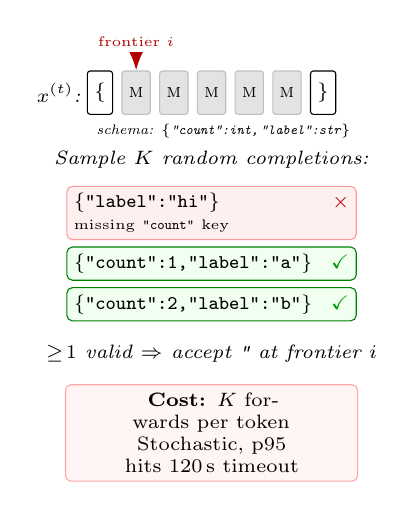
\begin{tikzpicture}[
  font=\footnotesize,>=Latex,
  tok/.style={draw,rounded corners=1pt,inner sep=2.5pt,minimum height=5.5mm,
              align=center,font=\scriptsize\ttfamily},
  mtok/.style={tok,fill=gray!22,draw=gray!50,font=\scriptsize},
  arr/.style={->,thick},
  samp/.style={draw,rounded corners=2pt,inner sep=2.5pt,font=\scriptsize,
                text width=3.5cm,align=left},
]
  \node[tok] (i0) at (0,0) {\{};
  \node[mtok,right=3pt of i0] (i1) {\textsc{m}};
  \node[mtok,right=3pt of i1] (i2) {\textsc{m}};
  \node[mtok,right=3pt of i2] (i3) {\textsc{m}};
  \node[mtok,right=3pt of i3] (i4) {\textsc{m}};
  \node[mtok,right=3pt of i4] (i5) {\textsc{m}};
  \node[tok,right=3pt of i5]  (i6) {\}};
  \node[font=\scriptsize\itshape,anchor=east] at (-0.12,0) {$x^{(t)}$:};
  \node[font=\tiny\itshape,anchor=west] at ($(i0.south west)+(0,-0.2)$)
    {schema: \texttt{\{"count":int,\,"label":str\}}};
  \draw[arr,red!70!black] (i1.north)++(0,.24) -- (i1.north);
  \node[font=\tiny,red!70!black,above=0.18cm of i1] {frontier $i$};

  \node[font=\scriptsize\itshape] (sl) at ($(i0)!0.5!(i6)+(0,-0.85)$)
    {Sample $K$ random completions:};
  \node[samp,fill=red!6,draw=red!40,anchor=north] (s1) at ($(sl.south)+(0,-0.1)$)
    {\texttt{\{"label":"hi"\}}\hfill\textcolor{red!70!black}{$\times$}\\
      {\tiny missing \texttt{"count"} key}};
  \node[samp,fill=green!6,draw=green!50!black,anchor=north] (s2) at ($(s1.south)+(0,-0.08)$)
    {\texttt{\{"count":1,"label":"a"\}}\hfill\textcolor{green!60!black}{$\checkmark$}};
  \node[samp,fill=green!6,draw=green!50!black,anchor=north] (s3) at ($(s2.south)+(0,-0.08)$)
    {\texttt{\{"count":2,"label":"b"\}}\hfill\textcolor{green!60!black}{$\checkmark$}};

  \node[font=\scriptsize\itshape,anchor=north] (dec) at ($(s3.south)+(0,-0.18)$)
    {$\geq\!1$ valid $\Rightarrow$ accept \texttt{"} at frontier $i$};
  \node[draw=red!35,fill=red!4,rounded corners=2pt,font=\scriptsize,
        text width=3.5cm,align=center,inner sep=3pt,anchor=north]
    at ($(dec.south)+(0,-0.15)$)
    {\textbf{Cost:} $K$ forwards per token\\Stochastic, p95 hits 120\,s timeout};
\end{tikzpicture}
\end{minipage}%
\hspace{2pt}%
\begin{minipage}[t]{0.49\linewidth}
\centering
{\small\bfseries Dgrammar:} {\small deterministic frontier masking}
\vspace{4pt}

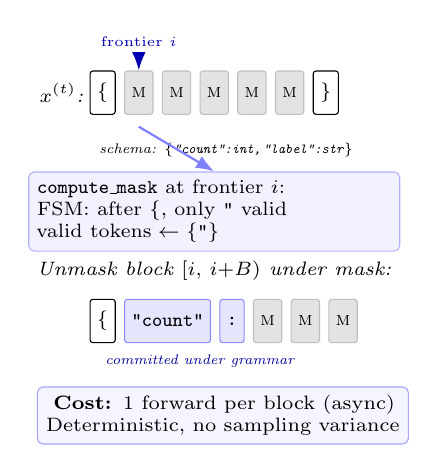
\begin{tikzpicture}[
  font=\footnotesize,>=Latex,
  tok/.style={draw,rounded corners=1pt,inner sep=2.5pt,minimum height=5.5mm,
              align=center,font=\scriptsize\ttfamily},
  mtok/.style={tok,fill=gray!22,draw=gray!50,font=\scriptsize},
  ctok/.style={tok,fill=blue!10,draw=blue!45},
  arr/.style={->,thick},
]
  \node[tok] (i0) at (0,0) {\{};
  \node[mtok,right=3pt of i0] (i1) {\textsc{m}};
  \node[mtok,right=3pt of i1] (i2) {\textsc{m}};
  \node[mtok,right=3pt of i2] (i3) {\textsc{m}};
  \node[mtok,right=3pt of i3] (i4) {\textsc{m}};
  \node[mtok,right=3pt of i4] (i5) {\textsc{m}};
  \node[tok,right=3pt of i5]  (i6) {\}};
  \node[font=\scriptsize\itshape,anchor=east] at (-0.12,0) {$x^{(t)}$:};
  \node[font=\tiny\itshape,anchor=west] at ($(i0.south west)+(0,-0.45)$)
    {schema: \texttt{\{"count":int,\,"label":str\}}};
  \draw[arr,blue!70!black] (i1.north)++(0,.24) -- (i1.north);
  \node[font=\tiny,blue!70!black,above=0.18cm of i1] {frontier $i$};

  \node[draw=blue!30,fill=blue!5,rounded corners=2pt,font=\scriptsize,
        text width=4.5cm,inner sep=3pt,anchor=north] (mask)
    at ($(i0)!0.5!(i6)+(0,-1)$)
    {\texttt{compute\_mask} at frontier $i$:\\
      FSM: after \texttt{\{}, only \texttt{"} valid\\
      $\mathrm{valid\ tokens} \gets \{\texttt{"}\}$};
  \draw[arr,blue!50] ($(i1.south)+(0,-0.15)$) -- (mask.north);

  \node[font=\scriptsize\itshape,anchor=north] (ul) at ($(mask.south)+(0,0)$)
    {Unmask block $[i,\,i{+}B)$ under mask:};

  \node[tok]  (c0) at (0,-2.9) {\{};
  \node[ctok,right=3pt of c0] (c1) {"count"};
  \node[ctok,right=3pt of c1] (c2) {:};
  \node[mtok,right=3pt of c2] (c3) {\textsc{m}};
  \node[mtok,right=3pt of c3] (c4) {\textsc{m}};
  \node[mtok,right=3pt of c4] (c5) {\textsc{m}};
  \node[font=\tiny\itshape,blue!60!black,anchor=north]
    at ($(c1)!0.5!(c2)+(0,-0.3)$) {committed under grammar};

  \node[draw=blue!35,fill=blue!4,rounded corners=2pt,font=\scriptsize,
        text width=4.5cm,align=center,inner sep=3pt]
    at ($(c0)!0.5!(c5)+(0,-1.2)$)
    {\textbf{Cost:} 1 forward per block (async)\\Deterministic, no sampling variance};
\end{tikzpicture}
\end{minipage}
\caption{One denoising step under schema \texttt{\{"count":int,\,"label":str\}}. \textbf{LAVE} \citep{lave2025} (left) samples $K$ random completions at each frontier token, accepting it only when $\geq\!1$ suffix is valid; stochastic and $K\!\times$ more expensive per token, hitting the 120\,s per-instance timeout on hard schemas. \textbf{Dgrammar} (right) runs \texttt{compute\_mask} on the incremental FSM state and unmasks an entire block under that mask in one forward pass, overlapped with the next mask computation; the result is deterministic. The figure is illustrative; LAVE's actual cost depends on its retry schedule and verifier policy (see \S\ref{sec:related}).}
\label{fig:denoise-compare}
\end{figure*}

\begin{table*}[t]
\small
\centering
\setlength{\tabcolsep}{4pt}
\begin{tabular}{llrrrrrrrr}
\toprule
\textbf{Split} & \textbf{Method} & \textbf{n} & \textbf{sch@1} & \textbf{mean} & \textbf{p50} & \textbf{p90} & \textbf{p95} & \textbf{p99} & \textbf{Timeout} \\
\midrule
\multicolumn{10}{c}{\textit{LLaDA-8B-Instruct}} \\
\midrule
easy   & Vanilla       & 558 & 64.2          & 2.58          & 2.48          & 3.23           & 3.38           & 4.02            & 0 \\
       & LAVE          & 558 & 82.3          & 24.95         & 2.74          & 120.00         & 120.00         & 120.00          & 83 \\
       & IG-CD$^\dagger$ & 449 & 79.1        & 2.58          & 2.31          & 3.97           & 5.12           & 9.60            & 0 \\
       & \textsc{Dgr.} & 558 & \textbf{94.1} & \textbf{3.14} & \textbf{2.71}  & \textbf{4.48}  & \textbf{5.36}  & \textbf{11.17}  & \textbf{0} \\
\cmidrule(lr){1-10}
medium & Vanilla       & 511 & 51.3          & 3.91          & 3.67          & 5.14           & 5.61           & 7.59            & 0 \\
       & LAVE          & 511 & 76.3          & 30.56         & 12.32         & 120.00         & 120.00         & 120.00          & 65 \\
       & IG-CD$^\dagger$ & 383 & 67.4        & 9.65          & 3.91          & 17.97          & 44.55          & 106.89          & 4 \\
       & \textsc{Dgr.} & 511 & \textbf{84.5} & \textbf{5.24} & \textbf{4.39}  & \textbf{8.56}  & \textbf{12.76} & \textbf{15.54}  & \textbf{0} \\
\cmidrule(lr){1-10}
hard   & Vanilla       & 269 & 24.9          & 9.30          & 7.52          & 15.33          & 17.69          & 25.45           & 0 \\
       & LAVE          & 269 & 53.2          & 45.01         & 22.42         & 120.00         & 120.00         & 120.00          & 56 \\
       & IG-CD$^\dagger$ & 245 & 38.8        & 39.97         & 14.82         & 120.00         & 120.00         & 120.19          & 50 \\
       & \textsc{Dgr.} & 269 & \textbf{54.3} & \textbf{24.17}& \textbf{19.46} & \textbf{46.50} & \textbf{54.44} & \textbf{86.21}  & \textbf{0} \\
\midrule
\multicolumn{10}{c}{\textit{Dream-7B}} \\
\midrule
easy   & Vanilla       & 552 & 65.0          & 1.20          & 0.98          & 2.26           & 2.45           & 2.62            & 0 \\
       & LAVE          & 552 & 83.5          & 31.18         & 10.28         & 120.00         & 120.00         & 120.00          & 65 \\
       & \textsc{Dgr.} & 552 & \textbf{94.0} & \textbf{5.29} & \textbf{3.27}  & \textbf{11.12} & \textbf{14.01} & \textbf{23.89}  & \textbf{0} \\
\cmidrule(lr){1-10}
medium & Vanilla       & 506 & 41.5          & 2.71          & 2.79          & 3.81           & 4.17           & 5.16            & 0 \\
       & LAVE          & 506 & 78.3          & 34.20         & 15.37         & 120.00         & 120.00         & 120.00          & 58 \\
       & \textsc{Dgr.} & 506 & \textbf{82.2} & \textbf{9.11} & \textbf{6.21}  & \textbf{17.55} & \textbf{21.18} & \textbf{44.20}  & \textbf{0} \\
\cmidrule(lr){1-10}
hard   & Vanilla       & 258 & 12.4          & 5.99          & 5.29          & 9.22           & 10.94          & 14.12           & 0 \\
       & LAVE          & 258 & 56.2          & 41.01         & 18.89         & 120.00         & 120.00         & 120.00          & 43 \\
       & \textsc{Dgr.} & 258 & \textbf{56.6} & \textbf{18.23}& \textbf{17.73} & \textbf{37.16} & \textbf{47.38} & \textbf{51.17}  & \textbf{0} \\
\bottomrule
\end{tabular}
\caption{JSB difficulty spectrum, B200, $T{=}128$. \textsc{Dgr.} denotes Dgrammar. Latencies in seconds; Timeout counts $\geq\!120$\,s instances. $n$ is matched-instance count after llguidance skips. $^\dagger$IG-CD \citep{mundler2025} runs on LLaDA only (no Dream backend); its CFG pipeline compiles just a subset of each split ($449/577$ easy, $383/586$ medium, $245/368$ hard, i.e.\ $22$--$35\%$ rejected), so its rows are over that compilable subset and schema@1 is not instance-matched to the other methods. Hyperparameters in App.~\ref{app:hyperparams}.}
\label{tab:main}
\end{table*}

\section{Method}
\label{sec:method}

Dgrammar runs the standard masked-diffusion loop but changes how grammar feedback is used. Instead of treating a violation as a rejection of the whole step, it preserves accepted tokens, repairs the first invalid frontier token under the same forward-pass logits, and uses parser feedback to control how aggressively the next step unmasks tokens. Algorithm~\ref{alg:dgrammar} gives the full step; Figure~\ref{fig:denoise-compare} contrasts it with LAVE.

\subsection{Prefix-Guided Selective Remasking}

The decoder maintains a left-to-right cursor $c$ into the generated region and a token-level matcher state \citep{llguidance}. After each batch unmask, \textsc{ExtendPrefix} feeds the contiguous non-mask suffix starting at $c$ to the matcher. If all tokens are consumed, $c$ advances. Otherwise, the first unconsumed position $p$ is the frontier violator; all earlier positions have already been accepted by the matcher.

The repair is local. Let $t_p$ be the rejected token at $p$. Dgrammar sets $\ell[p,t_p]=-\infty$, returns $x_p$ to \texttt{[MASK]}, takes the next argmax at $p$, and retries the matcher from the same accepted prefix. This loop uses the same forward-pass logits and costs only a vector argmax plus one matcher call per retry. It stops when the matcher accepts a replacement or when \texttt{max\_resamples} is reached. Tokens already accepted in the same batch are not re-decoded, so a single violation becomes a refinement target rather than a rollback to single-token decoding.

\subsection{Grammar-Gated Parallel Unmasking}

The batch size $K$ is a parser-controlled state variable updated by an additive-increase, multiplicative-decrease (AIMD) rule familiar from TCP congestion control: after a violation-free step we set $K\leftarrow \min(2K,K_{\max})$; after a violation we reset $K$ to one. This is analogous to confidence-adaptive schedules for diffusion decoding \citep{fastdllm2025}, but the signal is grammatical progress rather than softmax confidence. Easy spans therefore recover parallel unmasking quickly, while schema-sensitive regions such as delimiters, field names, and type-restricted values are decoded conservatively.

Grammar constraints are applied only at the current frontier. Before token selection, \textsc{ComputeMask} returns the vocabulary bias allowed by the matcher state at cursor $c$, and this bias is added to $\ell[c]$. Non-frontier positions are selected by the usual diffusion confidence rule. This frontier-only masking avoids constructing masks for every masked position in the block while still ensuring that the next token consumed by the parser is grammar-valid or becomes a selective-remasking target.

\subsection{Tail and Latency Control}

Two engineering choices keep constraint overhead from dominating the diffusion loop. First, mask construction for the current frontier is independent of the next model forward pass, so we launch \textsc{ComputeMask} on a background thread and join it after the forward pass. We fall back to synchronous mask computation only when a mid-step repair changes the matcher state. In our runs, this hides almost all mask construction latency behind GPU compute.

Second, if the diffusion loop exits before the matcher reaches an accepting state, we invoke a grammar-guided AR completion once from the current cursor, restricted to the unfinished suffix and refreshing the model logits at every emitted token under the grammar mask. In practice this mostly closes short tails such as braces or brackets; it is deliberately bounded, and failures from locally valid but schema-invalid completions are counted by the final \texttt{jsonschema.validate} metric. Algorithm~\ref{alg:dgrammar} summarizes the step-level procedure.

\begin{algorithm}[t]
\small
\caption{Dgrammar decoding step}
\label{alg:dgrammar}
\begin{algorithmic}[1]
\State \textbf{Input:} sequence $x$, cursor $c$, matcher $M$, batch $K$
\State Launch \textsc{ComputeMask}$(M)$ asynchronously $\to$ \texttt{pending}
\State $\ell \gets \textsc{Forward}(x)$ \Comment{forward pass}
\State \texttt{bias} $\gets$ join \texttt{pending}
\State $\ell[c] \gets \ell[c] + \texttt{bias}$ \Comment{frontier mask}
\State Choose top-$K$ confident masked positions, write argmax tokens
\State $c', v \gets \textsc{ExtendPrefix}(M, x, c)$
\If{$v \ne -1$} \Comment{violation at $v$}
  \State $\ell[v, x_v] \gets -\infty$; $x_v \gets [\text{MASK}]$
  \While{retries $<$ \texttt{max\_resamples}}
    \State $t \gets \arg\max \ell[v]$
    \If{$M.\textsc{TryConsume}([t]) = 1$} $x_v \gets t$; \textbf{break} \EndIf
    \State $\ell[v, t] \gets -\infty$
  \EndWhile
  \State $K \gets 1$
\Else
  \State $c \gets c'$; $K \gets \min(2K, K_{\max})$
\EndIf
\If{$M.\textsc{IsAccepting}()$} fill remaining with EOS \EndIf
\end{algorithmic}
\end{algorithm}

\section{Experiments}
\label{sec:experiments}

\subsection{Main JSB Results}

\paragraph{Setup.} We evaluate on JSONSchemaBench (JSB) medium\_test \citep{jsonschemabench2025}; after matcher compilation skips, 511 instances are common to all methods. All runs use an NVIDIA B200, $T{=}128$ steps, generation length 256, block length 32, temperature 0.2, and \texttt{seed=0}. We compare Dgrammar with \textsc{Vanilla} unconstrained generation and LAVE \citep{lave2025} on LLaDA-8B-Instruct \citep{llada2025} and Dream-v0-Instruct-7B (``Dream-7B'') \citep{dream2025}. Dgrammar uses one per-backbone setting for \texttt{max\_resamples} (500 for LLaDA, 2000 for Dream) and per-position AR autocomplete; LAVE uses its published default \texttt{max\_retry\_num\_total}$=$1000.

\paragraph{Metric.} We report \emph{schema@1}, the success of \texttt{jsonschema.validate} on the parsed output. This is stricter than the runner-internal grammar flag, which only checks the matcher's accepting state and can be inflated by truncated outputs.

\paragraph{Main results.} Table~\ref{tab:main} compares the systems. On LLaDA, \textsc{Vanilla} reaches only 51.3\% schema@1, while LAVE improves validity to 76.3\% at $7.8\times$ higher mean latency and with 65/511 timeouts. Dgrammar raises schema@1 to 84.5\%, runs $5.8\times$ faster than LAVE on mean latency and $9.4\times$ faster on p95, and has zero timeouts. Its mean latency is only $1.3\times$ above \textsc{Vanilla}, indicating that grammar enforcement adds little cost relative to diffusion forward passes. ETH/IG-CD~\citep{mundler2025} is not instance-matched: its CFG pipeline rejects $22$--$35\%$ of each split (Table~\ref{tab:main}, $\dagger$), and even on the schemas it compiles it trails Dgrammar at every difficulty ($79.1$ vs.\ $94.1$, $67.4$ vs.\ $84.5$, $38.8$ vs.\ $54.3$ schema@1) with $50/245$ timeouts on hard; we discuss it and DINGO in Limitations.


\subsection{Ablations and Failure Analysis}

Table~\ref{tab:ablation} ablates Dgrammar on the same 511 instances. Async overlap never changes validity (zero per-instance flips in both blocks); its latency effect depends on the fallback, because overlap can only hide mask construction behind the block-diffusion forward loop. Under the greedy block-completion fallback the tail stays in that loop, so overlap reduces mean and p95 latency by 21\% and 60\%. Under per-position AR autocomplete the tail is a sequence of one-forward-per-token steps that cannot be overlapped, so the async machinery only adds thread-synchronization overhead; its mean latency is therefore within noise of the no-overlap variant ($5.24$ vs.\ $4.97$\,s), with the overall system still dominated by the AR tail. Autocomplete is the main validity-recovery mechanism, with schema@1 dropping from 84.5\% to 75.7\% when it is disabled under the AR setting. Multi-token unmasking mainly saves forward passes: forcing $K_{\max}{=}1$ keeps validity nearly flat but raises mean latency by 144\% under AR autocomplete. Finally, \texttt{max\_resamples} is a validity/latency knob whose effect depends on the fallback: under greedy it trades validity for speed, while under AR autocomplete lower budgets shift work into slower per-token completion.

\begin{table}[!ht]
\small
\centering
\begin{tabular}{lrrr}
\toprule
\textbf{Config} & \textbf{schema@1} & \textbf{mean} & \textbf{p95} \\
\midrule
\multicolumn{4}{l}{\textit{AR autocomplete (Table~\ref{tab:main} setting)}} \\
Dgrammar (full)        & \textbf{84.5\%} & \textbf{5.24} & \textbf{12.76} \\
~~$-$ async overlap             & 84.5\%          & 4.97          & 12.69 \\
~~$-$ \textsc{Autocomplete}     & 75.7\%          & 5.94          & 11.13 \\
~~$K_{\max}{=}1$                & 84.0\%          & 12.79         & 37.30 \\
~~\texttt{max\_resamples}${=}100$ & 84.1\%        & 9.55          & 26.82 \\
~~\texttt{max\_resamples}${=}50$  & 83.6\%        & 11.55         & 31.49 \\
\midrule
\multicolumn{4}{l}{\textit{Greedy block-completion fallback}} \\
Dgrammar (full)        & 81.0\%          & 6.35          & 14.02 \\
~~$-$ async overlap             & 81.0\%          & 7.71          & 22.38 \\
~~$-$ \textsc{Autocomplete}     & 75.7\%          & 4.64          &  7.46 \\
~~$K_{\max}{=}1$                & 80.4\%          & 10.26         & 35.28 \\
~~\texttt{max\_resamples}${=}100$ & 77.3\%        & 4.81          &  9.36 \\
~~\texttt{max\_resamples}${=}50$  & 75.5\%        & 4.74          &  7.80 \\
\bottomrule
\end{tabular}
\caption{Component ablation on JSB medium\_test ($n{=}511$, LLaDA-8B-Instruct, B200, $T{=}128$, seed=0). Latencies in seconds. Top block uses per-position AR autocomplete (the Table~\ref{tab:main} setting); bottom block uses the greedy block-completion variant for comparison.}
\label{tab:ablation}
\end{table}

\begin{figure}[!t]
\centering
\resizebox{\linewidth}{!}{%
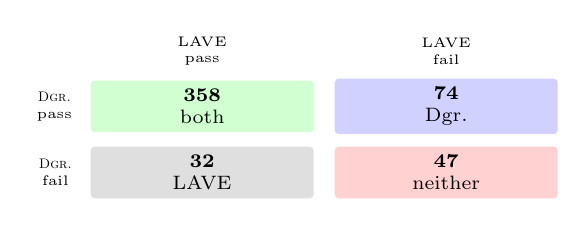
\begin{tikzpicture}[
  font=\scriptsize,
  cell/.style={draw=white,line width=0.5pt,rounded corners=1.5pt,
               minimum width=2.85cm,minimum height=0.62cm,align=center},
  lab/.style={font=\tiny,align=center},
  barlabel/.style={font=\tiny,anchor=east},
]
  \node[lab] at (2.55,0.55) {LAVE\\pass};
  \node[lab] at (5.65,0.55) {LAVE\\fail};
  \node[lab,anchor=east] at (1.02,-0.15) {\textsc{Dgr.}\\pass};
  \node[lab,anchor=east] at (1.02,-0.99) {\textsc{Dgr.}\\fail};
  \node[cell,fill=green!18,text=black] at (2.55,-0.15) {\textbf{358}\\both};
  \node[cell,fill=blue!18,text=black] at (5.65,-0.15) {\textbf{74}\\Dgr.};
  \node[cell,fill=gray!25,text=black] at (2.55,-0.99) {\textbf{32}\\LAVE};
  \node[cell,fill=red!18,text=black] at (5.65,-0.99) {\textbf{47}\\neither};
\end{tikzpicture}
}
\caption{Paired schema@1 outcomes on JSB medium\_test (LLaDA-8B-Instruct, $n{=}511$). Off-diagonal cells show instances solved by only one decoder.}
\label{fig:failure-breakdown}
\end{figure}

The paired outcomes in Figure~\ref{fig:failure-breakdown} show where the validity gains and remaining failures come from. Among the 511 common JSB medium\_test instances, Dgrammar and LAVE agree on 405 cases (358 both pass, 47 both fail). Dgrammar wins 74 cases that LAVE misses, while LAVE wins 32 cases that Dgrammar misses. Thus the improvement is not because one method dominates every schema, but because Dgrammar's wins are concentrated in LAVE's expensive failure mode: schemas where stochastic lookahead repeatedly rejects constrained continuations and often reaches the 120\,s timeout. On the 65 LAVE timeout instances, Dgrammar never times out.

The remaining 32 LAVE-only successes expose the main boundary of our method (\S\ref{app:dream-failures} gives the same decomposition for Dream). On these instances, LAVE's mean runtime is $21.8$\,s (max $87.3$\,s, well below the timeout), so they are genuine constraint-quality losses rather than easy cases LAVE happened to find first. Re-validating Dgrammar's failed outputs shows all of them fail at JSON parsing rather than schema validation: the median failed output is $578$ characters long, exceeding the $256$-token budget, so the dominant residual failure mode is tail closure on long-output schemas (App.~\ref{app:dream-failures}) rather than field selection. Lowering \texttt{max\_resamples} barely moves validity under the AR autocomplete fallback ($84.5$\%$\!\to\!84.1$\% at budget $100$, $\!\to\!83.6$\% at budget $50$); the cost shifts to latency instead, since more instances run out of resample budget and trigger the per-token AR completion (mean $5.24\!\to\!9.55\!\to\!11.55$\,s). Conversely, increasing the budget can recover validity on harder backbones, as in Dream medium\_test, but at a measurable latency cost. Dgrammar should therefore be read as a better validity--latency Pareto point, not as a universal validity winner over lookahead verification on every split.

\paragraph{Case study.} Instance \texttt{o83272} is representative of the timeout wins (App.~\ref{app:case}). Its schema contains enum and format-constrained fields such as \texttt{resource}, integer counts, and date strings. LAVE must verify a frontier token by drawing random completions; for an enum field this requires a free-form completion to hit a specific token such as \texttt{"CPU"}, so every lookahead batch fails and the instance reaches the 120\,s timeout. Dgrammar instead masks the frontier vocabulary to enum-valid tokens, completes the instance in 3.39\,s with zero resamples, and produces schema-valid output.

\paragraph{Empirical intervention rate.} Figure~\ref{fig:intervention} compares per-instance intervention counts on JSB medium\_test (LLaDA-8B). LAVE's lookahead retries have a long tail (median 16, mean 261, max 3334), with each retry costing $K{=}5$ extra forward passes. Dgrammar's selective remasks are much more compact in the body (median 1; 43.4\% of instances need zero resamples and complete the diffusion loop without any frontier repair) and bounded by \texttt{max\_resamples} in the tail; each remask is an argmax on existing logits, with no additional forward pass. The intervention machinery therefore engages rarely on most instances and, when it does, perturbs only the violating frontier token rather than the whole frontier scoring rule.

\vspace{\intextsep}
\vspace{1.5\intextsep}
\begin{center}
\centering
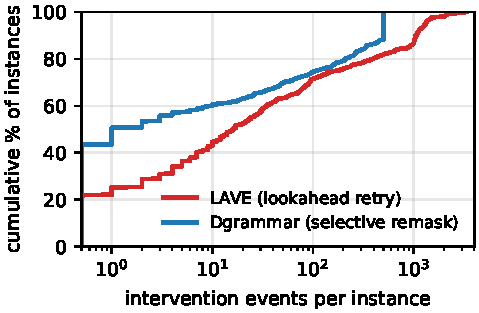
\includegraphics[width=\linewidth]{intervention_dist.pdf}
\captionof{figure}{Empirical CDF of intervention events per instance on JSB medium\_test (LLaDA-8B-Instruct, $n{=}511$). LAVE retries are lookahead-verification draws ($K{=}5$ forward passes each); Dgrammar resamples are selective remasks (no extra forward pass). Dgrammar's median is 1 vs.\ LAVE's 16; Dgrammar bounds its tail at \texttt{max\_resamples}$=$500.}
\label{fig:intervention}
\end{center}

\subsection{Transfer and Runtime Overhead}

\paragraph{Difficulty spectrum.} Across all three JSB splits and both backbones, Dgrammar matches or exceeds LAVE on validity while always running with zero timeouts. On LLaDA, the validity advantage is $+11.8$/$+8.2$/$+1.1$ pp on easy/medium/hard; on Dream the pattern is similar ($+10.5$/$+3.9$/$+0.4$ pp), with the gap narrowing on hard schemas where stochastic lookahead is more likely to find a valid completion. LAVE's timeout rate stays roughly stable across difficulty ($14.9\%$/$12.7\%$/$20.8\%$ on LLaDA), indicating its long-tail failure mode is structural (e.g., enum/format constraints) rather than tied to JSB's difficulty labels.

\begin{table}[!htbp]
\small
\centering
\setlength{\tabcolsep}{4pt}
\begin{tabular}{llrr}
\toprule
\textbf{Dataset} & \textbf{Method} & \textbf{syn@1} & \textbf{fun@1} \\
\midrule
\multicolumn{4}{c}{\textit{LLaDA-8B-Instruct}} \\
\midrule
JSON   & Vanilla       & 85.7          & 46.7 \\
JSON   & LAVE          & 98.5          & 52.9 \\
JSON   & \textsc{Dgr.} & \textbf{99.3} & 52.2 \\
\cmidrule(lr){1-4}
SMILES & Vanilla       & 65.3          & 2.4 \\
SMILES & LAVE$^{\!\ddagger}$ & 98.7    & 0.0 \\
SMILES & \textsc{Dgr.} & \textbf{100.0} & \textbf{3.0} \\
\midrule
\multicolumn{4}{c}{\textit{Dream-7B}} \\
\midrule
JSON   & Vanilla       & 86.8          & 49.6 \\
JSON   & LAVE          & 95.9          & 45.8 \\
JSON   & \textsc{Dgr.} & 94.8          & \textbf{45.2}\,$^{\!\dagger}$ \\
\cmidrule(lr){1-4}
SMILES & Vanilla       & 79.6          & \textbf{3.6} \\
SMILES & LAVE$^{\!\ddagger}$ & 99.4    & 0.0 \\
SMILES & \textsc{Dgr.} & \textbf{99.4} & 2.4 \\
\bottomrule
\end{tabular}
\caption{Cross-benchmark validity. JSON-Bench ($n{=}272$) and SMILES ($n{=}167$); B200, same hyperparameters as Table~\ref{tab:main}. SMILES syn@1 follows \citet{lave2025}'s CFG-acceptance metric; fun@1 is RDKit canonical equivalence. LAVE uses its published default (\texttt{max\_retry\_num\_total}$=$1000); the tuned $N{=}10,\tau{=}10$ in \citet{lave2025} gives higher fun@1 ($55.0$/$54.4$ on LLaDA/Dream JSON). $^{\dagger}$LAVE Dream-7B JSON timeouts $=8$; Dgrammar $=0$. $^{\ddagger}$LAVE SMILES syn@1 from \citet{lave2025} Table~1; that paper excludes SMILES from fun@1 (all methods round to $0\%$).}
\label{tab:cross}
\end{table}

\paragraph{Functional correctness.} On the JSON-Bench split (\texttt{json-mode-eval-extended}, $n{=}272$) used by LAVE \citep{lave2025}, Dgrammar's functional@1 (exact match against ground truth) is statistically indistinguishable from LAVE's: $52.2$ vs.\ $52.9$ on LLaDA-8B and $45.2$ vs.\ $45.8$ on Dream-7B (both within $0.7$\,pp; case-insensitive: $61.1$ vs.\ $61.0$ and similar pattern on Dream). Both also clear the unconstrained ceiling: \textsc{Vanilla}'s fun@1 is $46.7$/$49.6$ on LLaDA/Dream, so Dgrammar adds $+5.5$/$-4.4$ pp\footnote{The Dream regression is within the $0.7$\,pp gap to LAVE noted above and tracks LAVE's own behavior on this split, suggesting it reflects sampling variance under the temperature$=$$0.2$ setting rather than a constraint cost.} on top of the model's own success rate. Because LAVE applies grammar enforcement only as a stochastic verifier on top of the same base model, this match is the right reference point: it shows Dgrammar's deterministic frontier masking does \emph{not} cost semantic accuracy beyond the model's own ceiling. Latency, in contrast, drops $17$--$75$\% on LLaDA and $3\times$/$10\times$ (mean/p95) on Dream, with zero timeouts vs.\ LAVE's eight on Dream.

\paragraph{Cross-grammar transfer (SMILES).} To test that Dgrammar's algorithm is not specific to JSON-Schema, we plug in a CFG-mode checker (rustformlang-backed CFG/DFA intersection-emptiness) and run on \texttt{eth-sri/smiles-eval} ($n{=}167$, Table~\ref{tab:cross}). Dgrammar reaches $100.0$\% syn@1 on LLaDA-8B ($+34.7$ pp over \textsc{Vanilla}, also above LAVE's $98.7$\%) and $99.4$\% on Dream-7B (matching LAVE), confirming the algorithm transfers to non-JSON grammars. Functional@1 stays at $2$--$4$\,\% across all methods because the SMILES grammar accepts any single atom as a valid \texttt{Line}, and exact-match against a stereoisomeric reference is dominated by the model's chemistry knowledge rather than constraint enforcement; \citet{lave2025} likewise reports $0$\% functional on this split. The full Dgrammar pipeline transfers across backbones via only a per-model adapter (forward signature, mask/EOS token IDs, tokenizer); see Table~\ref{tab:cross}.

\begin{table}[!t]
\centering
\begin{tabular}{lr}
\toprule
\textbf{Operation} & \textbf{Mean} \\
\midrule
grammar check (per call)        & 0.15\,ms \\
mask compute (per call)         & 13.23\,ms \\
mask wait after async overlap   & 0.05\,ms \\
mask time saved (per instance)  & 1034\,ms \\
autocomplete fallback fires     & 26.2\% \\
\bottomrule
\end{tabular}
\caption{Per-operation overhead for Dgrammar on JSB medium\_test.}
\label{tab:overhead}
\end{table}

Table~\ref{tab:overhead} reports per-operation timing for Dgrammar on JSB medium\_test. The grammar check averages 0.15\,ms per call, three to four orders of magnitude below a forward pass. Mask construction averages 13.2\,ms but is overlapped with the forward pass on every step where the frontier is masked, saving on average about 1.0\,s per instance and reducing the observed mask wait to 0.05\,ms. The autocomplete fallback fires on 26.2\% of instances; its cost is bounded because it only completes the suffix that the diffusion loop failed to close. On the AR run (Table~\ref{tab:main}), the AR completion produces a median of $21$ tokens per fired instance (mean $72.6$, max $245$) and accounts for only $8.8$\% of all generated tokens, so most output is still produced by the multi-token diffusion loop.

\section{Conclusion}

We argued that per-token constraint overhead is a useful axis for comparing grammar-constrained decoders on DLMs, and built Dgrammar, a decoder that preserves multi-token unmasking while enforcing token-level grammar via incremental prefix checking and selective remasking. On JSONSchemaBench, Dgrammar both improves schema-valid rate over the strongest existing DLM baseline and reduces tail latency by an order of magnitude. The overhead breakdown suggests that, once mask construction is overlapped, the dominant systems risk is not grammar checking itself but extra model forwards caused by retries, fallbacks, or token-by-token commitment. We will release the full implementation, including the asynchronous mask overlap, AIMD $K_{\max}$ schedule, and matcher integration, upon publication.

\paragraph{Future directions.} Three extensions follow naturally: a stronger autocomplete fallback (short beam search or a learned tail-completion head) to narrow the long-output validity gap, integration with parallel-decoding accelerators \citep{fastdllm2025,dmax2025,chen2025dparallel} whose adaptive-$K$ schedules our mask-based repair should be compatible with, and scaling Dgrammar to larger CFGs (Python, C++) via vectorized DFA or sparse-transition compilation.

\section*{Limitations}

\paragraph{Coverage and grammar support.} We evaluate on two DLMs and three benchmark families. Table~\ref{tab:cross} shows transfer from JSON-Schema to SMILES via a CFG-mode checker, but we have not yet tested larger code grammars such as C++ or Python, where grammar size may dominate latency. Dgrammar also inherits llguidance's schema coverage: 75 recursive \texttt{\$ref+oneOf} JSB schemas cannot be compiled and are skipped by all methods. We include ETH/IG-CD \citep{mundler2025} in Table~\ref{tab:main} but it is not instance-matched: its regex backend rejects $22$--$35\%$ of each split (e.g.\ \texttt{\textbackslash/} URI escapes and null-bounded length quantifiers), and even on the schemas it does compile it trails Dgrammar at every difficulty while hitting $50/245$ timeouts on hard. Its implementation also targets LLaDA only, so we report no Dream numbers. We omit DINGO \citep{dingo2025} because no runnable implementation was released at submission time. Finally, all runs use a matched \texttt{seed=0}; multi-seed sweeps, LAVE hyperparameter sweeps, and grammar-size scaling are left for future work.

\paragraph{Algorithm and semantic ceiling.} The autocomplete fallback is the main correctness frontier; better fallbacks such as short beam search or learned completion heads may improve tail closure. Grammar constraints guarantee \emph{structural} validity, not semantic quality: valid outputs can still be empty arrays, empty objects, short strings, or otherwise uninformative, contributing to the gap between schema@1 and functional@1 (Table~\ref{tab:cross}). We also do not claim that Dgrammar samples from the constrained joint distribution; frontier-only masking is a limited bias, not a zero-bias procedure. In deployment, Dgrammar should be treated as a structural enforcement layer, with downstream semantic and safety checks applied as usual.

\bibliography{custom}

\appendix

\section{Hyperparameters}
\label{app:hyperparams}

Table~\ref{tab:hyperparams} lists shared hyperparameters across all methods on JSB medium\_test.

\begin{table}[h]
\small
\centering
\begin{tabular}{ll}
\toprule
\textbf{Hyperparameter} & \textbf{Value} \\
\midrule
Diffusion steps $T$       & 128 \\
Random seed               & 0 \\
Block length              & 32 \\
Generation length         & 256 \\
Remasking strategy        & low-confidence \\
Temperature               & 0.2 \\
Max resamples (LAVE)      & 1000 \\
Max resamples (Dgrammar) & 500 \\
$K_{\max}$ (multi-token unmask)   & 8 \\
Per-instance timeout      & 120\,s \\
\bottomrule
\end{tabular}
\caption{Shared hyperparameters for benchmark runs.}
\label{tab:hyperparams}
\end{table}

\section{Dataset and Instance Filtering}
\label{app:data}

JSB medium\_test contains 586 schemas; 75 are excluded from all comparisons because llguidance rejects them at compile time (recursive \texttt{\$ref+oneOf} structures). LAVE returns immediately with \texttt{valid=false} (\texttt{"Prompt does not conform to grammar"}); Dgrammar silently skips them via the same llguidance guard. Since all methods behave identically on these instances, including them would inflate failure counts without providing meaningful comparison. All headline numbers are reported on the matched $n{=}511$ subset.

\section{Case Study: Instance \texttt{o83272}}
\label{app:case}

We examine instance \texttt{o83272}, a cluster resource allocation schema where LAVE times out and Dgrammar succeeds in a single pass with zero resamples. The schema requires fields with type-constrained values: \texttt{resource} (enum string), integer fields (\texttt{nodes}, \texttt{processors}, \texttt{ppn}, \texttt{percent\_allocated}), and date strings.

\paragraph{Why LAVE fails (timeout, 120\,s, no output).} LAVE commits a token only if all $K$ randomly sampled completions yield a grammar-valid continuation. For enum or typed fields, this requires a random natural-language completion to match a specific technical token (e.g., \texttt{"CPU"} for \texttt{resource}). LLaDA-8B assigns negligible probability mass to such targeted strings as free continuations, so every lookahead batch fails. LAVE cannot commit even the first constrained token and hits the 120\,s wall without producing output.

\paragraph{Dgrammar (valid, 0 resamples, 3.39\,s).} Frontier masking restricts the vocabulary at each position to the set of tokens permitted by the matcher. For \texttt{resource}, only the enum-valid tokens are unmasked; for integer and date fields, only digits and the appropriate format tokens are exposed. Because the matcher guides every token choice, no violation occurs and the selective-remasking path is never triggered. The output is complete and schema-valid:

\begin{center}\footnotesize
\begin{tabular}{l}
\verb|{|\\
\verb|  "resource": "CPU",|\\
\verb|  "nodes": 4,|\\
\verb|  "processors": 16,|\\
\verb|  "ppn": 4,|\\
\verb|  "start_date": "2023-10-01",|\\
\verb|  "end_date": "2023-10-31",|\\
\verb|  "percent_allocated": 75,|\\
\verb|  "comments": "..."|\\
\verb|}|\\
\end{tabular}
\end{center}

\paragraph{Summary.} This is the general failure mode of stochastic lookahead on enum and format-constrained fields: the probability of a random completion matching a specific technical string is effectively zero, so LAVE never commits. Frontier masking sidesteps this entirely. Among the 65 instances where LAVE times out on JSB medium\_test, 46 succeed under Dgrammar with similar mechanics; the median Dgrammar time on these 46 instances is 5.2\,s, a $23\times$ speedup over the LAVE timeout.

\section{Dream Failure Decomposition}
\label{app:dream-failures}

To check why Dgrammar's margin over LAVE is narrower on Dream-7B medium/hard than on LLaDA, we bucketed every invalid output on the matched JSB intersections ($n{=}506$/$258$) as \emph{empty}, \emph{parse\_error}, or \emph{schema\_error}. Empty outputs are timeout/give-up cases; parse errors are truncated or malformed JSON; schema errors are parsed JSON objects rejected by \texttt{jsonschema}. Table~\ref{tab:dream-fail} reports the counts.

\begin{table}[h]
\small
\centering
\setlength{\tabcolsep}{4pt}
\begin{tabular}{lllrrr}
\toprule
\textbf{Method} & \textbf{Split} & \textbf{Fails} & \textbf{Empty} & \textbf{Parse} & \textbf{Schema} \\
\midrule
LAVE   & medium & 110 & 33 & 77 & 0 \\
\textsc{Dgr.} & medium & 90  & 0  & 90 & 0 \\
\cmidrule(lr){1-6}
LAVE   & hard   & 113 & 40 & 73 & 0 \\
\textsc{Dgr.} & hard   & 120 & 0  & 120 & 0 \\
\bottomrule
\end{tabular}
\caption{Dream-7B failure decomposition on JSB medium ($n{=}506$) and hard ($n{=}258$). Both decoders have zero schema errors; all failures occur before validation. Dgrammar eliminates empty timeout outputs, but its remaining failures are long parse errors (mean $577$/$761$ chars), beyond the $256$-token budget. Thus the Dream hard regime mostly tests generation length rather than constraint quality.}
\label{tab:dream-fail}
\end{table}

\section{EOS-Validity vs.\ Schema-Validity}
\label{app:format}
\label{app:eos-validity}

A subtle but important distinction motivates our choice of metric. The runner-internal \texttt{valid} flag tests only whether an EOS token is present and no \texttt{[MASK]} remains before it; this is necessary for grammar-valid output but not sufficient when schemas carry \emph{format} constraints (e.g., \texttt{format:\,"uuid"}, \texttt{format:\,"uri"}) that llguidance compiles into the token automaton.

For example, on a schema requiring \texttt{target:\,\{type:\,string,\,format:\,"uuid"\}}, Dgrammar can emit a token sequence whose individual tokens each satisfy the automaton's prefix condition, but whose concatenation, e.g., \texttt{"12000e1TestCaseCanceledEvent"}, does not match the full RFC\,4122 pattern. The EOS check passes; \texttt{jsonschema.validate} on the parsed output fails. We therefore report only \emph{schema@1}, the result of \texttt{jsonschema.validate}, in all main tables; the same definition is used for LAVE. This is the same metric used by JSONSchemaBench \citep{jsonschemabench2025}.

\section{Engineering Details}
\label{app:engineering}

\textbf{AIMD $K_{\max}$ schedule.} Each block starts at $K{=}1$. After every successful unmask we set $K\!\gets\!\min(2K, K_{\max})$ (multiplicative increase); on a grammar violation we drop to $K{=}1$ (additive collapse) and repair the frontier via selective remasking. With $K_{\max}{=}8$, $T{=}128$, and block length $32$, this converges to $K{=}2$--$3$ on average ($\bar K\!\approx\!1.96$ in our runs).

\textbf{Async mask overlap.} \texttt{compute\_mask} runs on a CPU worker thread and is launched immediately after the previous step's logits are committed. The next forward pass starts on the GPU without waiting; when its logits arrive, the worker's mask is already done, so observed mask wait drops from $13.2$\,ms (compute-bound) to $0.05$\,ms (sync-bound).

\textbf{Per-backbone adapter.} The runner abstracts model-specific bits behind three hooks: (i) \texttt{forward\_fn}, which on Dream applies a one-position causal shift to align logits with the masking convention; (ii) \texttt{(mask\_id, eos\_id)} token IDs; (iii) the tokenizer. No other code paths differ across LLaDA-8B and Dream-7B.

\section{AR Autocomplete Suffix Length}
\label{app:ac-dist}

Among the $123$ instances ($24.1$\% of $511$) where AR autocomplete fires on the LLaDA-8B AR run, the suffix length distribution is heavy-tailed: median $21$ tokens, p75 $130$, p95 $224$, max $245$ (mean $72.6$). The bulk of fires close short tails (braces, brackets, trailing keys); the tail beyond $\sim$$200$ tokens corresponds to schemas where the diffusion loop exhausts \texttt{max\_resamples} early and AR completes most of the output. Across all $511$ instances, AR contributes $8{,}928$ tokens vs.\ $92{,}069$ from the diffusion loop ($8.8$\%).

\end{document}
